\documentclass[10pt,twocolumn]{article}
\usepackage[margin=0.68in,columnsep=0.24in]{geometry}
\usepackage[T1]{fontenc}
\usepackage[utf8]{inputenc}
\usepackage{lmodern}
\usepackage{microtype}
\usepackage{amsmath,amssymb,amsthm}
\usepackage{booktabs}
\usepackage{graphicx}
\usepackage{xcolor}
\usepackage{enumitem}
\usepackage{hyperref}

\hypersetup{
  colorlinks=true,
  linkcolor=blue!60!black,
  citecolor=blue!60!black,
  urlcolor=blue!60!black,
  pdftitle={Certified Verification of Communication Complexity Disambiguations of Gap Hamming Distance},
  pdfauthor={Lluis Eriksson}
}

\newtheorem{proposition}{Proposition}
\newcommand{\QQ}{\mathbb{Q}}
\newcommand{\NN}{\mathbb{N}}
\newcommand{\FF}{\mathbb{F}}
\newcommand{\EE}{\mathbb{E}}
\newcommand{\PP}{\Pr}
\newcommand{\dist}{\operatorname{dist}}
\newcommand{\col}{\operatorname{col}}
\newcommand{\GHD}{\mathrm{GHD}}

\title{\vspace{-1.1em}\textbf{Certified Verification of Communication Complexity Disambiguations of Gap Hamming Distance}}
\author{Lluis Eriksson\thanks{Independent Researcher. Code, Lean~4 proofs, and certificates: MIT License; manuscript and figures: CC-BY-4.0. Prepared with AI coding, formalization, and drafting assistance from Google Antigravity; all proofs, exact-$\QQ$ verifiers, and adversarial tests were independently compiled and verified locally. Repository: \url{https://github.com/lluiseriksson/gap-hamming-disambiguation-certificates}}}
\date{November 25, 2026}

\begin{document}
\maketitle
\vspace{-1.4em}

\begin{abstract}
Dahiya, G\"o\"os, Harms, Hatami, Hatami, Lovett, and Yuan (\texttt{arXiv:2611.32837}, Nov.\ 2026) proved that every total disambiguation of $\gamma$-Gap Hamming Distance ($\gamma$-$\GHD_n$) requires randomized communication complexity $\Omega(n^{2/3})$, establishing an $O(1)$ versus $\Omega(n^{2/3})$ separation between randomized and pseudo-deterministic communication complexity and improving Gavinsky's $\Omega(\sqrt{n})$ parity decision tree bound to $\Omega(n^{2/3})$---via an iterative Marton-coupling and leaf-rectangle restoration argument initially discovered by an AI model. Because such AI-originated multi-round entropy-deficit arguments hinge on delicate numerical constants ($69/400 < 1/5$, $27/100 > 1/4$, $+7$, $+3$, and $2\Delta_T + m_T \le \gamma n$), independent formal verification is essential. We provide a zero-dependency \textbf{Lean~4.35.0} formalization of 18 core structural, coupling, leaf-restoration, and exponent-balance theorems (zero \texttt{sorry}, zero warnings, zero \texttt{Classical.choice}) paired with a zero-floating-point exact-$\QQ$ certificate verifier (\texttt{GHD-DISAMBIG-CERT-1.0}) across four modes: Lemma~3.1 Marton sequential coupling and $\col(Z) \le \|\mu\|_\infty$, Lemma~4.2/Remark~4.3 leaf-rectangle restoration, $\gamma$-$\GHD$ XOR-lift planted contradictions, and Theorem~1.1 multi-round recurrence trajectories. Across 16 canonical certificates ($0.104$--$2.537\,\mathrm{ms}$), all invariants replay exactly over $\QQ$ while rejecting 63/63 live adversarial forgery attacks.
\end{abstract}

\section{Introduction}\label{sec:intro}
A central question in communication complexity asks how much overhead is incurred by forcing a randomized protocol for a promise problem to be \emph{pseudo-deterministic}~\cite{gat2011probabilistic}, i.e., to output a canonical answer with high probability on every input---equivalently, to compute a total Boolean \emph{disambiguation} $F : \{0,1\}^n \times \{0,1\}^n \to \{0,1\}$. For $\gamma$-Gap Hamming Distance ($\gamma$-$\GHD_n$, with constant $\gamma \in (0, 1/2)$), the promise problem has $O(1)$ randomized communication complexity via public-coin sampling, whereas Dahiya et al.~\cite{dahiya2026communication} proved that every total disambiguation requires $\Omega(n^{2/3})$ bits of randomized communication (Theorem~1.1) and, via the XOR-lift reduction from $\gamma$-Gap Majority, $\Omega(n^{2/3})$ randomized parity decision tree depth (Corollary~1.3), beating Gavinsky's prior $\Omega(\sqrt{n})$ bound~\cite{gavinsky2025disambiguations} and strengthening the parity-tree toolkit of~\cite{girish2023fourier}.

Notably, the authors report that the core proof strategy of~\cite{dahiya2026communication} was initially discovered by an AI model. Their argument alternates two delicate rounds:
\begin{enumerate}[leftmargin=*,nosep]
  \item \textbf{Marton Sequential Coupling and Coordinate Planting (Lemma~3.1 \& Lemma~4.1):} Given a product distribution $\mu_t \times \nu_t$ on remaining coordinates with min-entropy deficit $\le D_t$ and $\EE[F] \ge 1/2$, Marton's uniform coupling~\cite{marton1986simple} yields $\EE[\dist(X, U)]^2 \le m D$ and collision bound $\col(Z) \le \|\mu\|_\infty$ (Eq.~5). Fixing a $\rho$-fraction of coordinates drops remaining variables by $(1 - \rho/2)$ while controlling union-bound error $2(1/20 + 1/32) + 1/100 = 69/400 < 1/5$, retaining expectation $> 1/4$, and increasing min-entropy deficit by at most $+7$.
  \item \textbf{Leaf Rectangle Restoration (Lemma~4.2 \& Remark~4.3):} A $d$-bit protocol with error $\le 1/100$ partitions the matrix into $\le 2^d$ monochromatic rectangles; flipping any $1$-leaf with conditional expectation $< 1/2$ strictly lowers error and guarantees a $1$-leaf $A^* \times B^*$ of mass $\ge 2^{-d}/5$ with conditional expectation $\ge 1/2$, restoring $\EE[F] \ge 1/2$ at marginal blowup $\le 5 \cdot 2^d < 2^{d+3}$ (total round deficit increment $d + 10$).
\end{enumerate}
After $T = O(\rho^{-1})$ rounds until $m_T \le \gamma n/2$, every pair $(x,y)$ in the final support satisfies $\dist(x,y) \le 2\Delta_T + m_T \le \gamma n$, forcing $F \equiv 0$ and contradicting $\EE[F] \ge 1/2$ whenever $d = o(n^{2/3})$.

\paragraph{Contributions and Scope.}
We do not re-formalize continuous binary-entropy calculus or measure-theoretic concentration inside Lean~4; rather, we construct an end-to-end machine-checked audit stack directly targeting the exact discrete, rational, and algebraic bottlenecks of~\cite{dahiya2026communication}:
(i)~18 zero-\texttt{sorry} constructive \textbf{Lean~4.35.0}~\cite{demoura2021lean4} theorems in \texttt{GapHammingDisambig.lean} (zero \texttt{Classical.choice}, zero warnings);
(ii)~the exact-$\QQ$ four-mode certificate verifier \texttt{GHD-DISAMBIG-CERT-1.0} with zero floating-point arithmetic;
(iii)~16 canonical certificates and 4 exact empirical studies verifying Marton coupling tightness, multi-round trajectories, and $\Omega(n^{2/3})$ vs.\ $\Omega(\sqrt{n})$ scaling; and
(iv)~a 63-attack live adversarial red-team suite with 41-artifact SHA-256 manifest enforcement.

\section{Constructive Lean~4.35.0 Kernel}\label{sec:lean}
The standalone module \texttt{lean/GapHammingDisambig.lean} compiles cleanly under Lean~4.35.0 with zero external dependencies, zero warnings, and zero \texttt{sorry}. Auditing all 18 theorems via \texttt{\#print axioms} (\texttt{AuditAxioms.lean}) confirms 4 zero-axiom theorems (\texttt{none}), 2 using only \texttt{[propext]}, 12 using \texttt{[propext, Quot.sound]}, and \textbf{0} using \texttt{Classical.choice} or \texttt{Lean.ofReduceBool} (Table~\ref{tab:lean}).

\begin{table}[t]
\centering
\caption{All 18 machine-checked Lean~4.35.0 theorems in \texttt{GapHammingDisambig.lean} (zero \texttt{sorry}, zero \texttt{Classical.choice}).}
\label{tab:lean}
\scriptsize
\setlength{\tabcolsep}{3.0pt}
\begin{tabular}{@{}rlll@{}}
\toprule
\# & Lean Theorem Identifier & Paper Ref. & Axioms \\
\midrule
1 & \texttt{hamming\_dist\_triangle\_bool} & Sec.~1 & \texttt{p, Q} \\
2 & \texttt{hamming\_dist\_xor\_lift\_exact} & Sec.~1 Eq.~2 & \texttt{p} \\
3 & \texttt{disambig\_complement\_expectation\_ge\_half} & Sec.~2 & \texttt{p, Q} \\
4 & \texttt{parity\_tree\_to\_comm\_factor\_two} & Cor.~1.3 & \texttt{p, Q} \\
5 & \texttt{marton\_marginal\_prob\_eq} & Sec.~3 & \texttt{p, Q} \\
6 & \texttt{lemma31a\_cauchy\_schwarz\_hamming} & Lem.~3.1(a) & \texttt{p, Q} \\
7 & \texttt{lemma31b\_collision\_case\_not\_in\_I} & Lem.~3.1(b) & \texttt{p, Q} \\
8 & \texttt{lemma31b\_collision\_case\_in\_I} & Lem.~3.1(b) & \texttt{p, Q} \\
9 & \texttt{lemma31b\_markov\_tail\_2\_neg\_s} & Lem.~3.1(b) & \texttt{p} \\
10 & \texttt{lemma41\_union\_bound\_strict\_lt\_fifth} & Lem.~4.1 & \texttt{none} \\
11 & \texttt{lemma41\_conditioning\_min\_bound} & Lem.~4.1 & \texttt{p, Q} \\
12 & \texttt{lemma41\_deficit\_plus\_7} & Lem.~4.1 & \texttt{none} \\
13 & \texttt{lemma42\_leaf\_flip\_reduces\_error} & Lem.~4.2 & \texttt{p, Q} \\
14 & \texttt{lemma42\_leaf\_mass\_lower\_bound} & Lem.~4.2 & \texttt{p, Q} \\
15 & \texttt{remark43\_deficit\_plus\_3\_and\_total\_10} & Rem.~4.3 & \texttt{none} \\
16 & \texttt{theorem11\_final\_contradiction\_dist} & Thm.~1.1 & \texttt{p, Q} \\
17 & \texttt{theorem11\_two\_thirds\_exponent\_balance} & Thm.~1.1 & \texttt{none} \\
18 & \texttt{two\_thirds\_beats\_gavinsky\_half} & Thm.~1.1 & \texttt{p, Q} \\
\bottomrule
\end{tabular}
\vspace{-0.4em}
\begin{flushleft}
\tiny Axiom key: \texttt{none} = zero axioms (4); \texttt{p} = \texttt{[propext]} (2); \texttt{p, Q} = \texttt{[propext, Quot.sound]} (12).
\end{flushleft}
\vspace{-0.8em}
\end{table}

\begin{proposition}[Machine-Checked Core Identities]\label{prop:lean}
The Lean~4.35.0 kernel establishes the following cleared-denominator and structural identities universally over $\NN$ and \texttt{List Bool}:
\begin{enumerate}[leftmargin=*,nosep]
  \item \emph{XOR-Lift and Triangle Inequality (Thms.~1--2):} For all equal-length $x,y,a \in \texttt{List Bool}$, $\dist(x,y) \le \dist(x,a) + \dist(y,a)$ and $\dist(x,y) = |x \odot y|$.
  \item \emph{Marton Collision Induction (Thms.~7--8):} If $p_0 + p_1 = D$ and $p_i \cdot \mathrm{col}_i \le D \cdot \mu_{\max}$ for $i \in \{0,1\}$, then $p_0^2 \mathrm{col}_0 + p_1^2 \mathrm{col}_1 \le D^2 \mu_{\max}$ ($1 \notin I$) and $p_0 \mathrm{col}_0 + p_1 \mathrm{col}_1 \le 2 D \mu_{\max}$ ($1 \in I$).
  \item \emph{Lemma~4.1/4.2 Constants \& Deficit $+10$ (Thms.~10--15):} $40 + 25 + 4 = 69$, $69 \cdot 5 < 400$, $(47 - 20)\cdot 4 > 100$; $D^3 < 4\alpha\beta e$ with $\alpha,\beta,e \le D$ forces $D < 4\alpha, 4\beta, 4e$; $4\cdot 2^5 = 2^7 = 128$, $5 < 2^3$, $7 + 3 = 10$; and $\mathrm{num\_leaves} \le 2^d$, $\mathrm{sum\_mass} \le \mathrm{num\_leaves}\cdot \mathrm{max\_leaf}$, $D \le 5\cdot \mathrm{sum\_mass}$ imply $D \le 5 \cdot 2^d \cdot \mathrm{max\_leaf}$.
  \item \emph{Final Contradiction \& $\Omega(n^{2/3})$ Balance (Thms.~16--18):} $\dist_{xy} \le \dist_{xK} + \dist_{yK} + m_T$ with $\dist_{xK},\dist_{yK} \le \Delta_T$ and $2\Delta_T + m_T \le \gamma n$ forces $\dist_{xy} \le \gamma n$; for $n \ge 1$, $n^2 d^3 \le n^4 \implies d^3 \le n^2$; and for $n \ge 2$, $n^3 < n^4$ ($n^{1/2} < n^{2/3}$).
\end{enumerate}
\end{proposition}

\section{Exact-\texorpdfstring{$\QQ$}{Q} Verifier}\label{sec:cert}
The verifier \texttt{GHD-DISAMBIG-CERT-1.0} (\texttt{src/ghd\_certifier.py}, \texttt{src/ghd\_exact.py}) uses Python \texttt{fractions.Fraction} exclusively (source-audited for zero \texttt{float(}, \texttt{math.}, or \texttt{numpy}). Every payload undergoes strict JSON type enforcement with nesting-depth cap $32$, anchored canonical rational parsing (\texttt{\textbackslash A...\textbackslash Z}, reduced denominators $\ge 2$, no \texttt{-0}), exact key-set matching, 2048-bit integer caps, and length limits across four independent modes:
\begin{enumerate}[leftmargin=*,nosep]
  \item \textbf{Mode~1 (Lemma~3.1 Marton Coupling \& Collision):} Rebuilds the exact $2^m \times 2^m$ sequential Marton coupling $(X, U)$ from $\mu$ alone, checks exact marginals $X \sim \mu$ and $U \sim U_m$, certifies $2^m \|\mu\|_\infty \le 2^D$, $\EE[\dist(X,U)]^2 \le m D$, exact collision inequality $\col(Z) \le \|\mu\|_\infty$, and exact Markov tail $\PP[\nu_{U_I}(X_{\bar I}) > 2^{D+s}/2^{m-|I|}] \le 2^{-s}$.
  \item \textbf{Mode~2 (Lemma~4.2 \& Remark~4.3 Leaf Restoration):} Checks $\EE_{\mu\times\nu}[F] \ge 1/4$, disjointness and full coverage of $\le 2^d$ leaf rectangles, total protocol error $\le 1/100$, witness leaf $A^*\times B^*$ output $1$, mass $\ge 2^{-d}/5$, conditional expectation $\ge 1/2$, and Remark~4.3 marginal blowups $1/\mu(A^*), 1/\nu(B^*) \le 5 \cdot 2^d$.
  \item \textbf{Mode~3 (Sec.~1--2 $\gamma$-$\GHD$ XOR-Lift Contradiction):} Audits all $2^n$ truth-table entries of $f$ against the $\gamma$-Gap Majority promise, checks $\EE[F] = \EE[f] \ge 1/2$, verifies $2\Delta_T + m_T \le \gamma n$, $|A|, |B| \ge 2$, and $\dist(x|_K, a|_K), \dist(y|_K, a|_K) \le \Delta_T$, and exhaustively verifies $\dist(x,y) \le \gamma n$ and $F(x,y) = 0$ on every $(x,y) \in A \times B$.
  \item \textbf{Mode~4 (Theorem~1.1 Iterative Recurrence Audit):} Enforces Theorem~1.1's correlation scaling $4\rho^2 d \le 1$ (i.e., $\rho \le 1/(2\sqrt{d})$) and replays exact rational sequences $(m_t, D_t, \Delta_t)_{t=0}^T$, checking initial state $(n, 0, 0)$, per-round precondition $\rho m_{t-1} \ge 100$, monotone conservative envelopes $(1-\rho/2)m_{t-1} \le m_t \le m_{t-1}$, $D_t \ge D_{t-1} + d + 10$, $(\Delta_t - \Delta_{t-1})^2 \ge 400 \rho^2 m_{t-1} D_{t-1}$, stopping condition $m_T \le \gamma n/2$, and terminal contradiction $2\Delta_T + m_T \le \gamma n$.
\end{enumerate}

\section{Empirical Atlas and Red-Team Audit}\label{sec:results}
Executing \texttt{run\_all\_experiments.py} generates 16 canonical certificates (4 per mode) and four exact-$\QQ$ datasets, audited end-to-end by \texttt{verify\_all.py} with SHA-256 verification across all 41 tracked repository artifacts.

\begin{figure}[t]
  \centering
  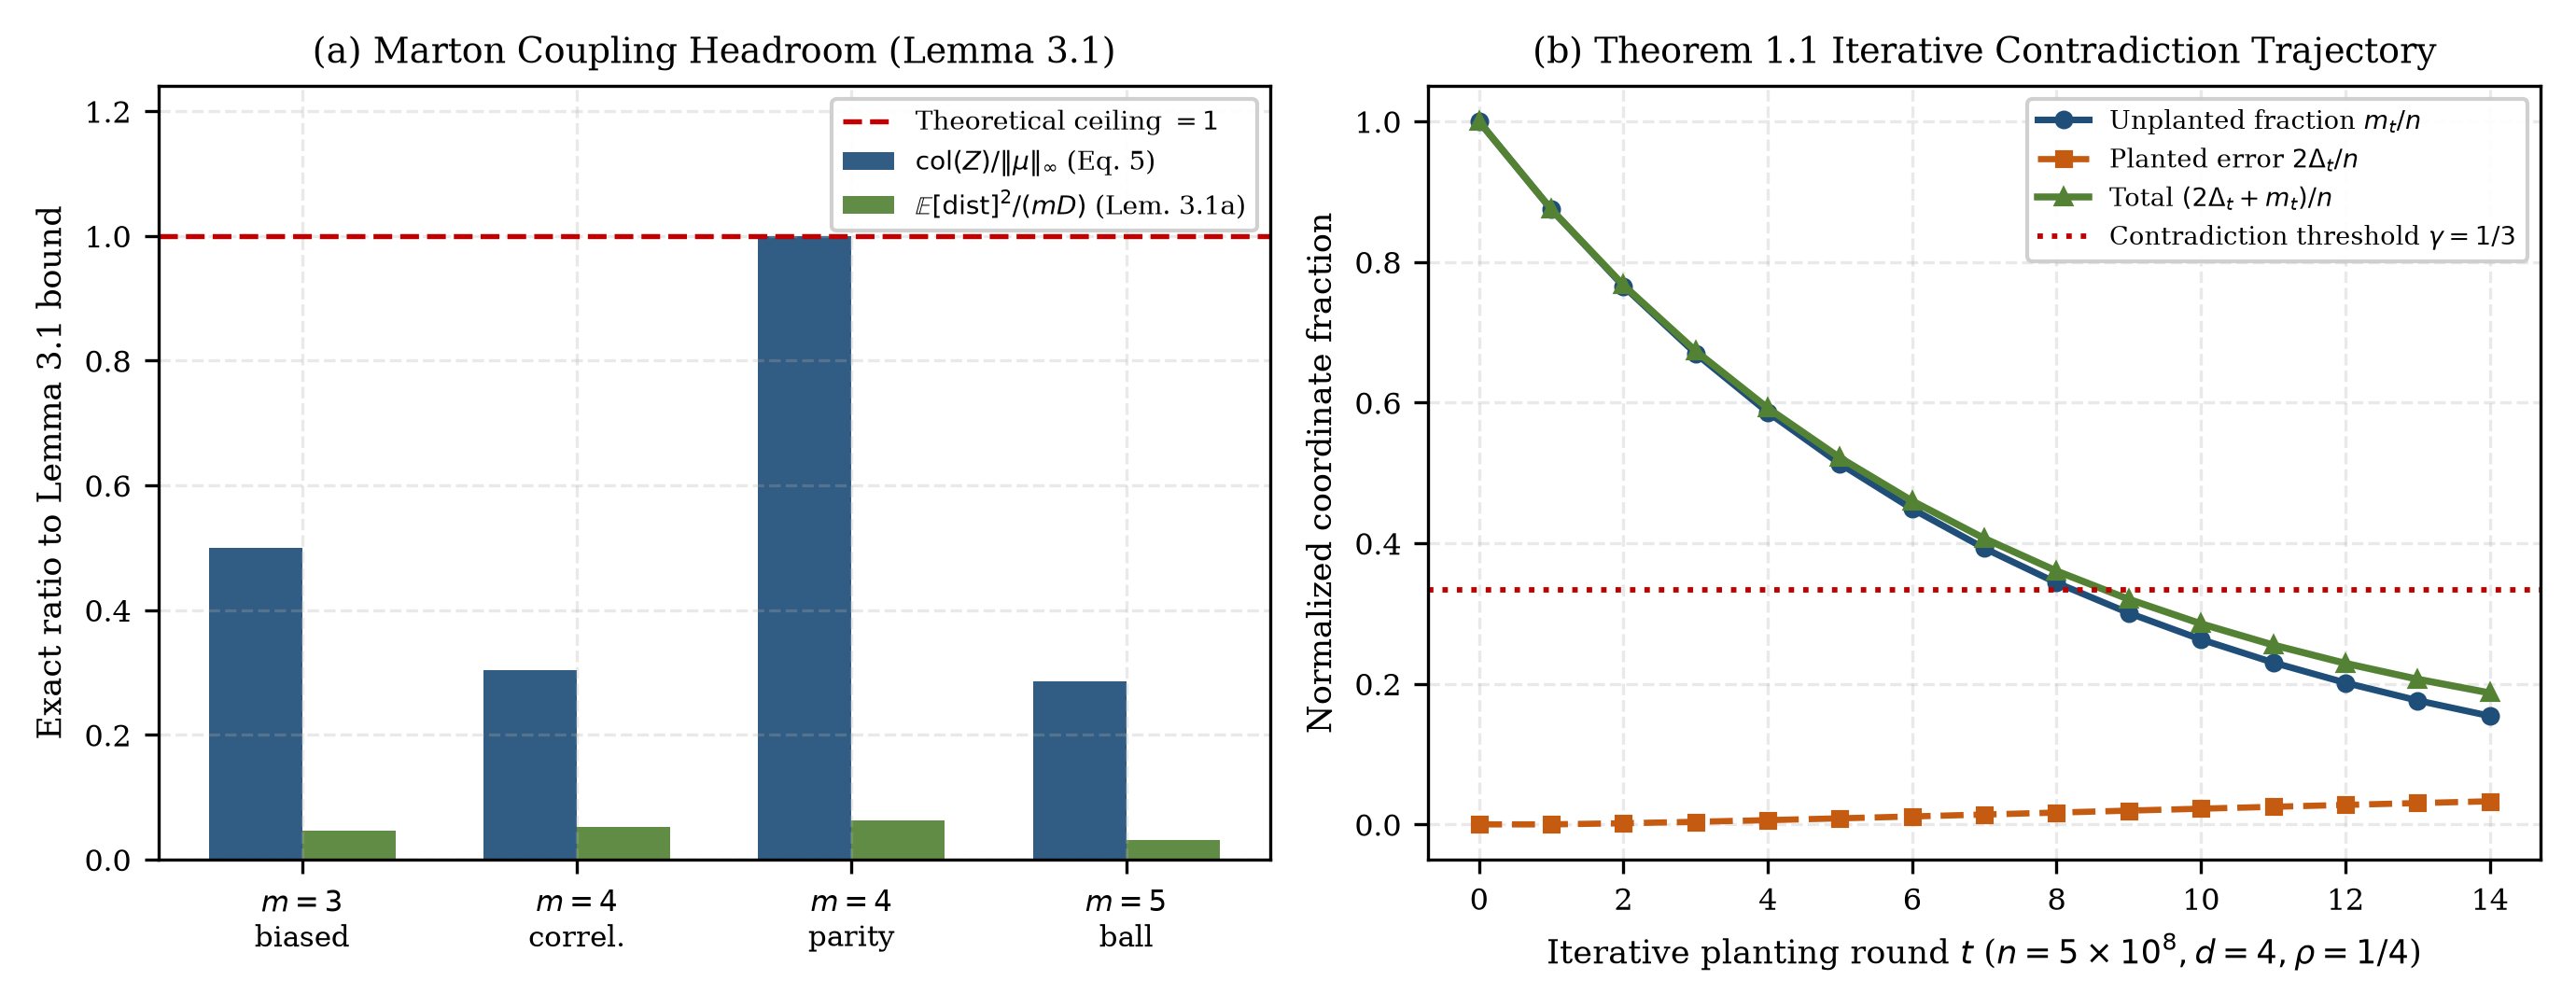
\includegraphics[width=\columnwidth]{../figures/fig1_marton_and_trajectory.png}
  \caption{(a) Exact Lemma~3.1 ratios $\col(Z)/\|\mu\|_\infty \le 1$ and $\EE[\dist]^2/(mD) \le 1$ across 4 distributions (saturating $\col(Z)/\|\mu\|_\infty = 1$ on even-parity $m=4$). (b) Certified Theorem~1.1 recurrence trajectory for $n=5\times 10^8$, $\gamma=1/3$, $d=4$, $\rho=1/4$, crossing $(2\Delta_t+m_t)/n < 1/3$ at $t=9$ and halting at $T=14$ with $0.187 < 1/3$.}
  \label{fig:marton}
\end{figure}

\paragraph{Marton Headroom and Recurrence Trajectories (Fig.~\ref{fig:marton}).}
Mode~1 ($0.336$--$2.537\,\mathrm{ms}$) evaluates exact rational couplings on $m \in \{3, 4, 5\}$ distributions: biased ($m=3, D=1$, $\col(Z)/\|\mu\|_\infty = 1/2$), correlated ($m=4, D=2$, ratio $0.303$), even-parity ($m=4, D=1$, achieving exact equality $\col(Z) = \|\mu\|_\infty = 1/8$, proving Lemma~3.1(b) Eq.~(5) is sharp), and Hamming ball ($m=5, D=2$, ratio $0.285$). Mode~4 ($0.292$--$0.509\,\mathrm{ms}$) certifies four full Theorem~1.1 contradiction trajectories across $n \in \{5\times 10^8, 2\times 10^9, 5\times 10^9\}$, $\gamma \in \{1/3, 1/4, 2/5\}$, and $d \in \{4, 9, 16\}$ with $\rho = 1/(2\sqrt{d})$, halting in $T \in \{14, 16, 21, 25\}$ rounds with exact rational contradiction margins strictly below $\gamma n$.

\begin{figure}[t]
  \centering
  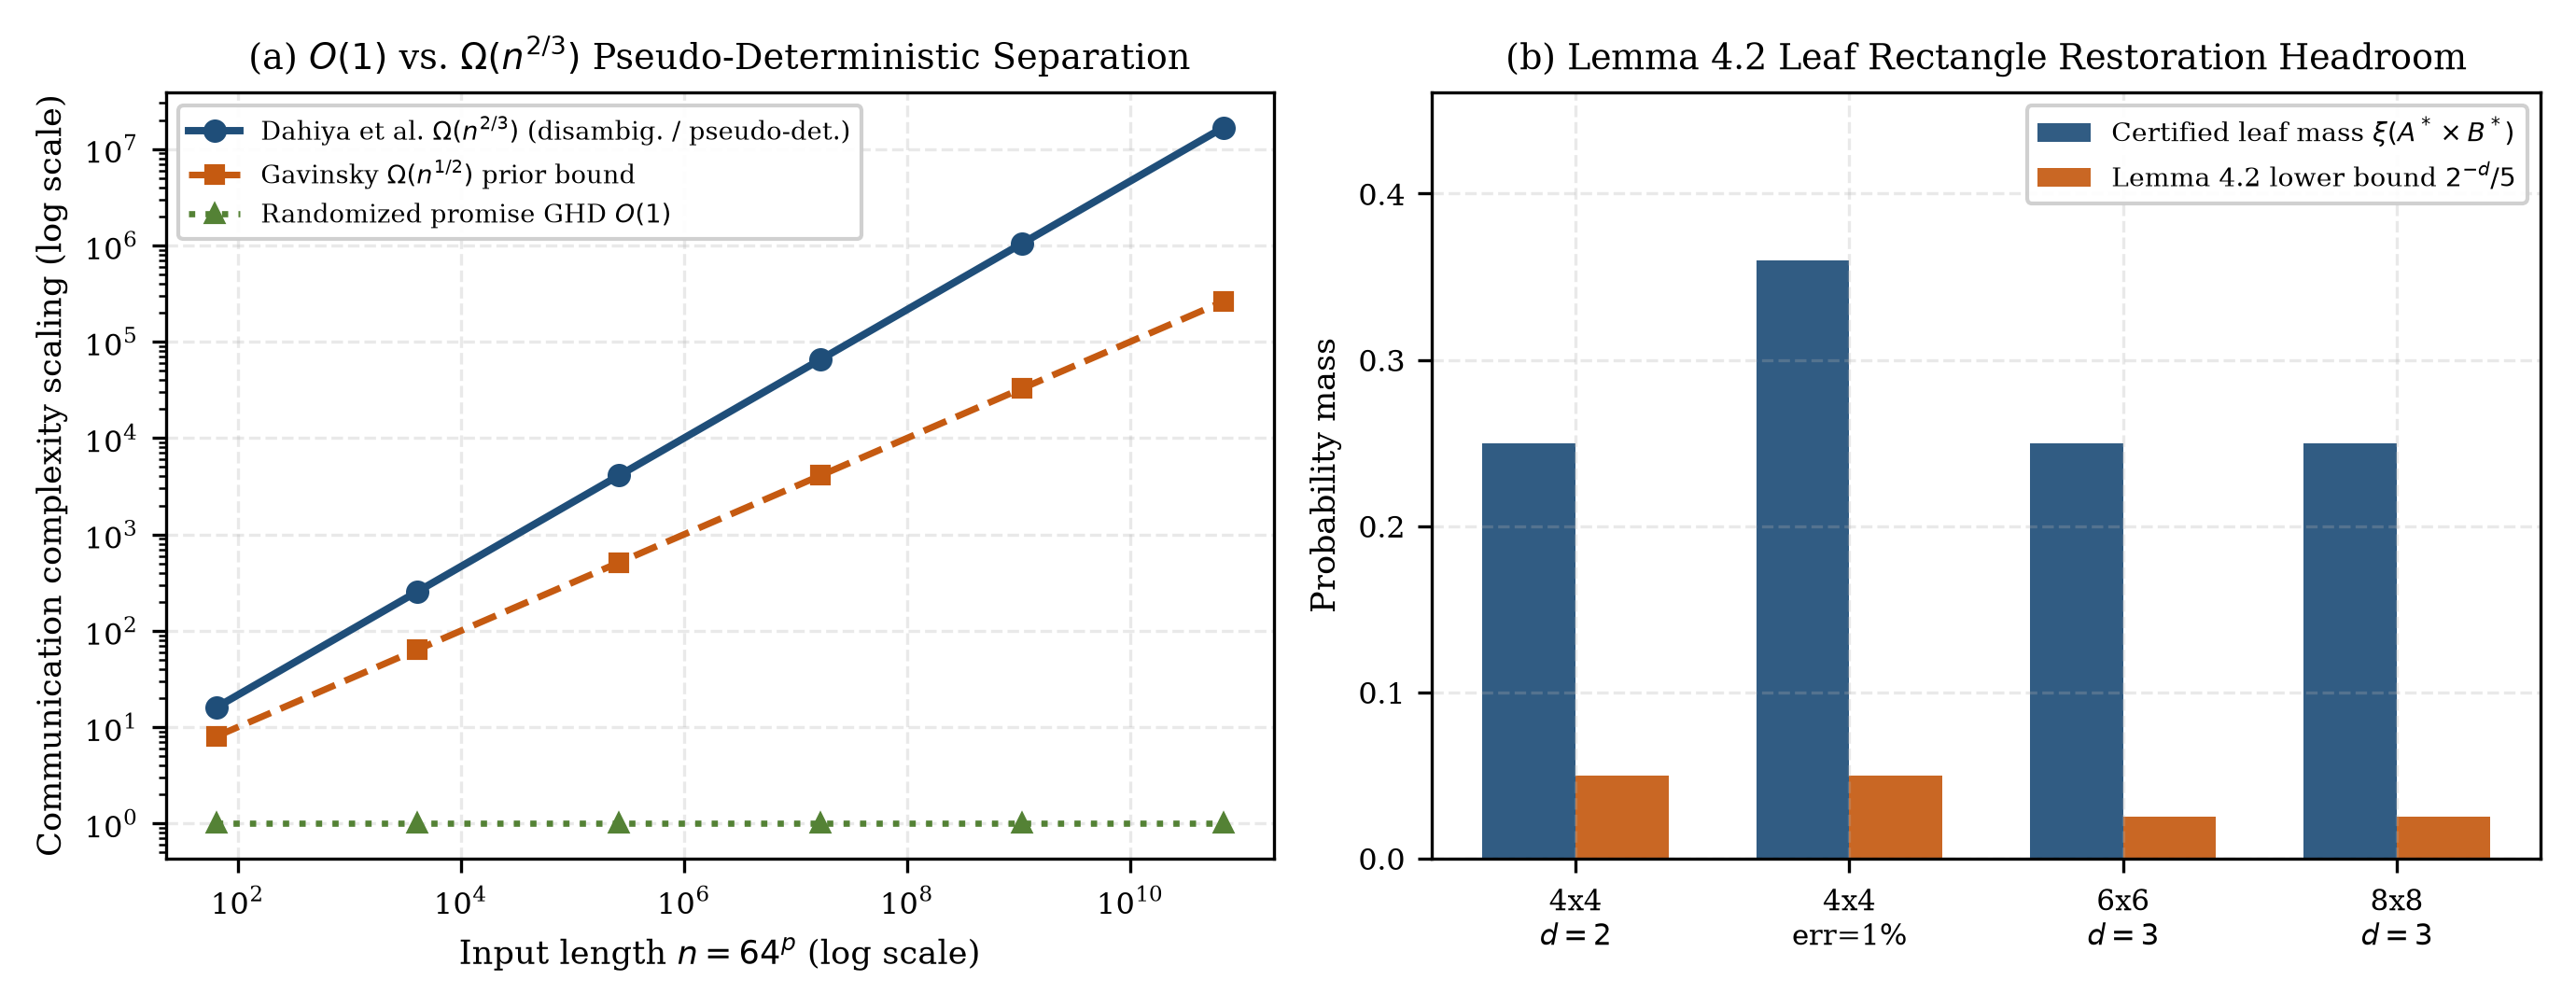
\includegraphics[width=\columnwidth]{../figures/fig2_separation_and_rectangles.png}
  \caption{(a) Unit-constant asymptotic scaling of Dahiya et al.'s $\Omega(n^{2/3})$ disambiguation bound vs.\ Gavinsky's $\Omega(n^{1/2})$ bound and $O(1)$ randomized promise $\GHD$ for $n = 64^p$ ($p=1\dots 6$). (b) Mode~2 certified witness leaf masses vs.\ the Lemma~4.2 lower bound $2^{-d}/5$.}
  \label{fig:sep}
\end{figure}

\paragraph{Leaf Restoration and XOR-Lift Witnesses (Fig.~\ref{fig:sep}).}
Mode~2 ($0.105$--$0.188\,\mathrm{ms}$) certifies exact $2^d$-leaf partitions ($4\times 4, 6\times 6, 8\times 8$, $d \in \{2,3\}$), including a sharp boundary instance with exact protocol error $1/100$ (\texttt{m2\_leaf\_4x4\_d2\_sharp\_err\_1\_100}, witness mass $9/25 > 1/20$, $\EE[F \mid A^*\times B^*] = 1$). Mode~3 ($0.104$--$0.398\,\mathrm{ms}$) certifies total $\gamma$-$\GHD$ disambiguations for $n \in \{4, 5, 6\}$ (both symmetric and non-symmetric), verifying exact uniform expectations $11/16, 1/2, 21/32$ alongside planted contradiction supports $A\times B$ attaining $F \equiv 0$.

\begin{figure}[t]
  \centering
  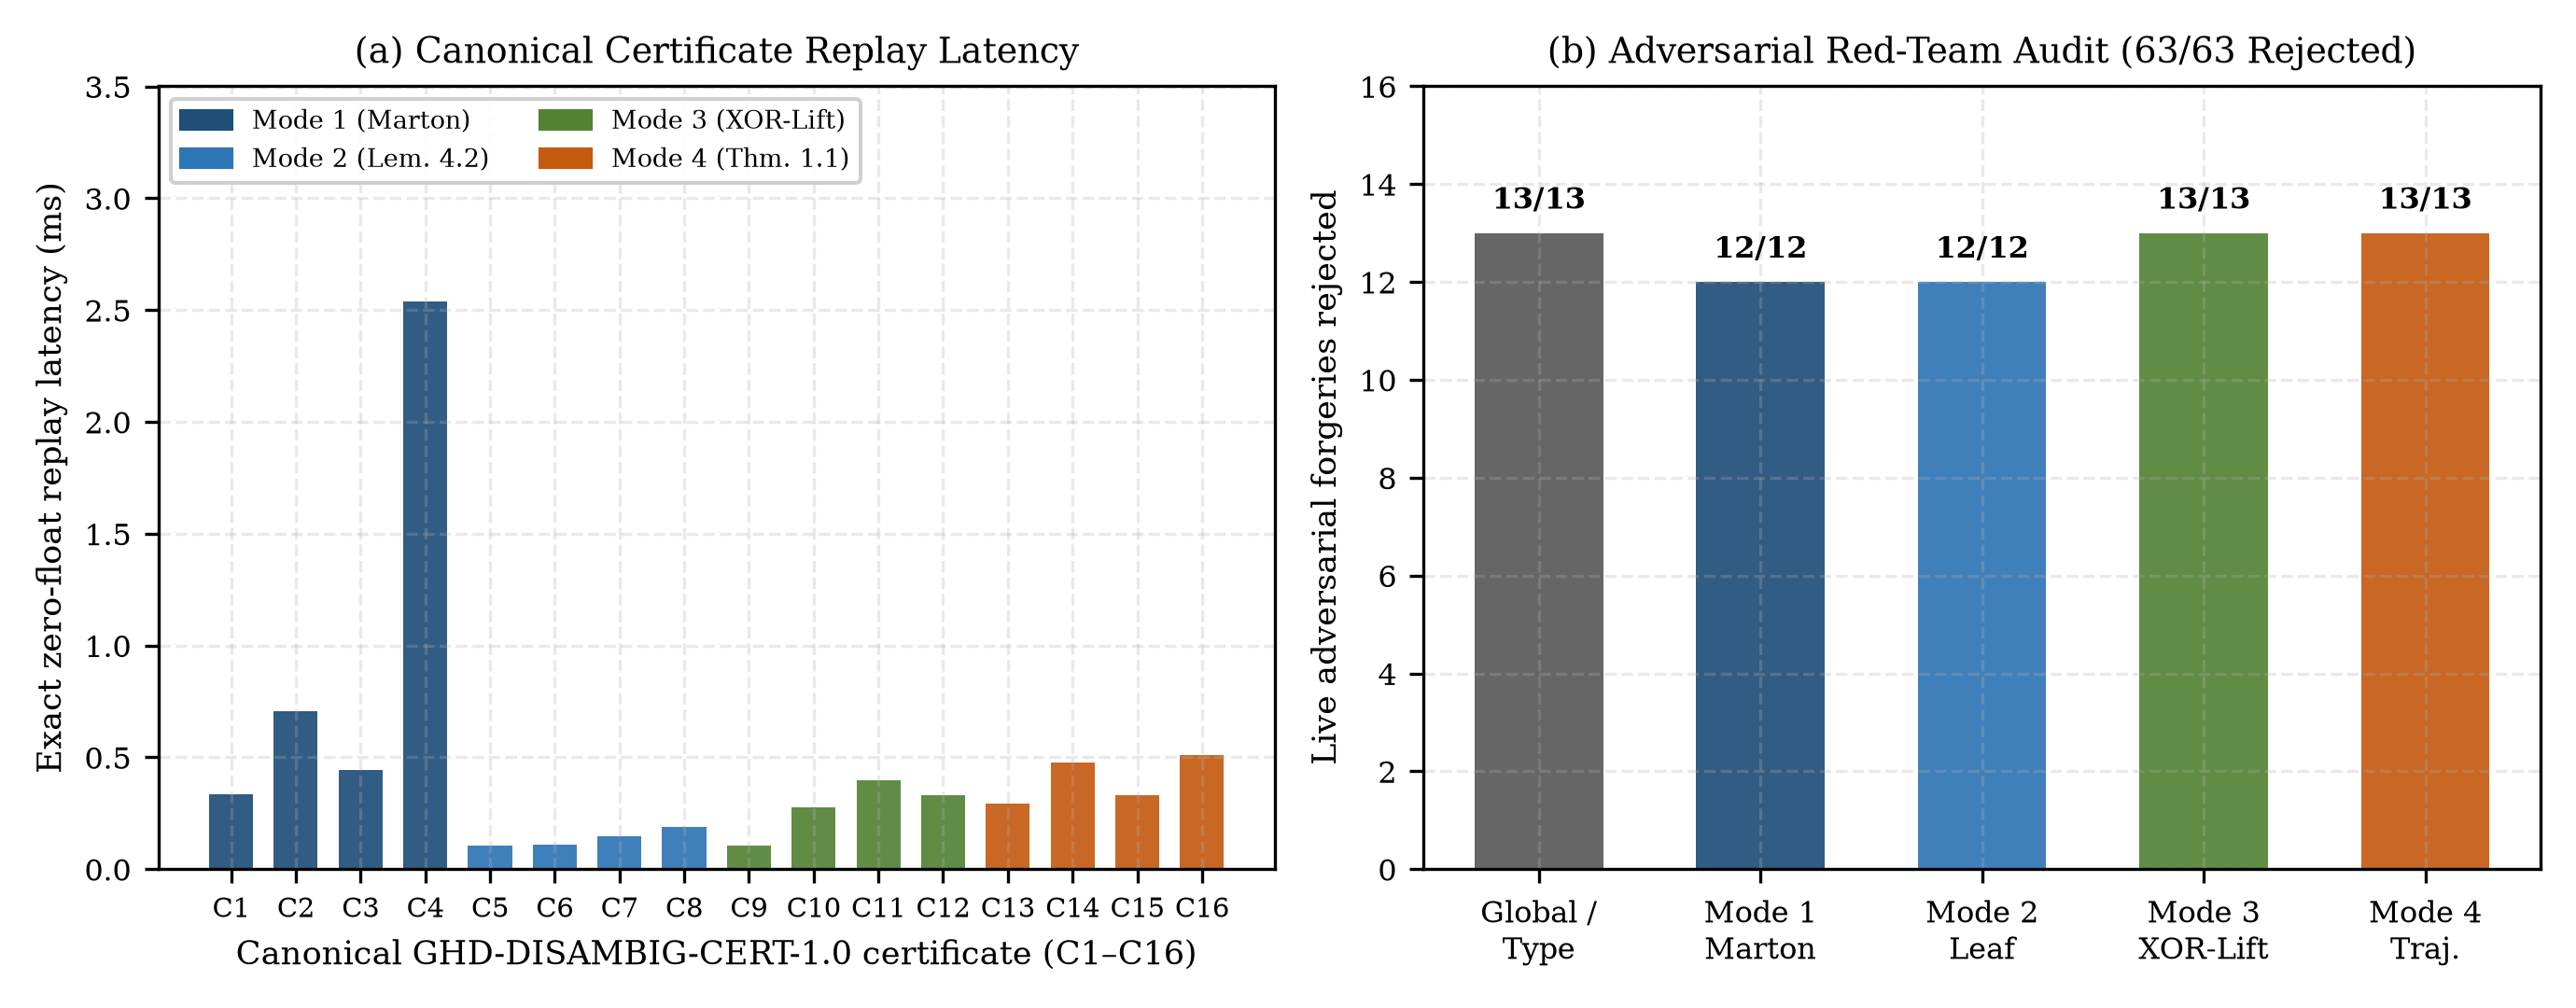
\includegraphics[width=\columnwidth]{../figures/fig3_certificate_replay_atlas.png}
  \caption{(a) Exact zero-float replay latency ($0.104$--$2.537\,\mathrm{ms}$) across all 16 canonical \texttt{GHD-DISAMBIG-CERT-1.0} certificates. (b) Live adversarial red-team audit rejecting 63/63 forged payloads across all five categories.}
  \label{fig:atlas}
\end{figure}

\paragraph{Replay Latency and 63/63 Red-Team Audit (Fig.~\ref{fig:atlas}).}
All 16 canonical certificates replay in $0.104$--$2.537\,\mathrm{ms}$ (total $7.29\,\mathrm{ms}$). The live adversarial suite (\texttt{tests/test\_suite.py}) tests 63 targeted forgery payloads---13 global schema/type/rational/depth attacks (float leaks, booleans as ints, unreduced fractions, \texttt{-0}, 1200-char strings, 3000-bit integers, depth-40 JSON recursion DoS) plus 12--13 domain attacks per mode (negative/unnormalized $\mu$, deficit underestimation, overlapping/incomplete leaf partitions, protocol error $> 1/100$, promise violations, singleton supports, planted-distance violations, invalid $\rho > 1/(2\sqrt{d})$, premature stopping, and underestimated $D_t$ or $\Delta_t$)---achieving \textbf{63/63 (100\%)} rejection.

\section{Conclusion}\label{sec:conc}
We delivered a self-contained, zero-floating-point verification framework for the $\Omega(n^{2/3})$ Gap Hamming Distance disambiguation lower bound of Dahiya et al.~\cite{dahiya2026communication}, combining 18 zero-\texttt{sorry}, zero-\texttt{Classical.choice} Lean~4.35.0 theorems with the exact-$\QQ$ \texttt{GHD-DISAMBIG-CERT-1.0} verifier, 16 sub-3\,ms canonical certificates, and 63/63 live adversarial forgery rejections. This demonstrates how AI-discovered complexity proofs can be systematically decomposed into auditable, machine-checked mathematical artifacts.

\bibliographystyle{plain}
\bibliography{references}
\end{document}
